\section{Results}
\label{sec:results}

\subsection{Main results on the held-out week}

Table~\ref{tab:main} reports the preregistered test results. At the 60-second horizon the base rate is 2.29\%. The XGBoost champion reaches an ROC-AUC of 0.866 and a PR-AUC of 0.112, and its top 1\% of observations has a precision of 14.6\%, 6.3 times the base rate. At the 300-second horizon the base rate is 2.73\%; the champion reaches 0.845 and 0.117, and its top 1\% has a precision of 16.2\%, 5.9 times the base rate. These figures are close to those on the validation week, where the champion scored 0.873 at 60 seconds. PR-AUC was higher on the test week (0.112 versus 0.092), largely because surges were more common that week (2.29\% versus 1.78\% of observations).

\begin{table}[t]
\centering
\caption{Preregistered test-week results. P@$k$ is the precision among the top $k$ of observations by score. The last column gives validation-week ROC-AUC and PR-AUC for reference. Bold marks the best value in a column within each horizon.}
\label{tab:main}
\tabsize
\setlength{\tabcolsep}{4pt}
\begin{tabular}{lccccccc}
\toprule
 & \multicolumn{6}{c}{Test week (preregistered, scored once)} & Validation \\
\cmidrule(lr){2-7}\cmidrule(lr){8-8}
Model & ROC-AUC & PR-AUC & P@0.1\% & P@0.5\% & P@1\% & P@2\% & ROC / PR \\
\midrule
\multicolumn{8}{l}{\emph{Onset within 60 s; base rate 2.29\%}} \\
XGBoost (champion) & 0.866 & \textbf{0.112} & 16.3\% & 15.4\% & 14.6\% & 16.0\% & 0.873 / 0.092 \\
LightGBM (tuned) & 0.866 & 0.108 & 13.0\% & 13.4\% & 13.2\% & 14.7\% & 0.873 / 0.090 \\
Logistic regression (L2) & \textbf{0.870} & 0.110 & 15.0\% & 14.3\% & 14.5\% & 14.8\% & 0.858 / 0.076 \\
Transformer & 0.852 & 0.095 & 10.5\% & 12.8\% & 12.6\% & 11.5\% & 0.858 / 0.077 \\
Age + curve XGBoost & 0.842 & 0.093 & 10.0\% & 10.6\% & 10.2\% & 9.8\% & 0.854 / 0.076 \\
\addlinespace
\multicolumn{8}{l}{\emph{Onset within 300 s; base rate 2.73\%}} \\
XGBoost (champion) & \textbf{0.845} & \textbf{0.117} & 17.1\% & 15.9\% & 16.2\% & 17.2\% & 0.858 / 0.098 \\
LightGBM (tuned) & 0.844 & 0.116 & 16.4\% & 16.1\% & 16.2\% & 16.5\% & 0.856 / 0.095 \\
Logistic regression (L2) & 0.845 & 0.114 & 15.7\% & 15.4\% & 16.1\% & 16.2\% & 0.834 / 0.078 \\
Transformer & 0.829 & 0.099 & 11.2\% & 12.9\% & 13.4\% & 12.4\% & 0.841 / 0.082 \\
Age + curve XGBoost & 0.818 & 0.097 & 11.2\% & 10.9\% & 11.0\% & 10.6\% & 0.836 / 0.080 \\
\bottomrule
\end{tabular}

\end{table}

The comparison between models is the more surprising result (Table~\ref{tab:deltas}). The champion clearly beats the Transformer, by 0.014 in ROC-AUC and 0.018 in PR-AUC at 60 seconds, with similar margins at 300 seconds, and it beats the age-and-curve model by 0.024 and 0.020. It does not clearly beat logistic regression. At 60 seconds, logistic regression has a slightly \emph{higher} ROC-AUC, by 0.0045, while the champion keeps a small PR-AUC advantage of 0.0028 whose interval nearly touches zero. At 300 seconds the two are tied on ROC-AUC, and the champion leads on PR-AUC by 0.0033. The tuned LightGBM is within 0.002 ROC-AUC of the champion at both horizons.

\begin{table}[t]
\centering
\caption{Paired differences on the test week (champion minus each model), with 95\% confidence intervals from a token-clustered bootstrap (2,000 replicates).}
\label{tab:deltas}
\tabsize
\begin{tabular}{llcc}
\toprule
Horizon & Champion minus & $\Delta$ROC-AUC [95\% CI] & $\Delta$PR-AUC [95\% CI] \\
\midrule
60 s & Logistic regression & $-$0.0045 [$-$0.0068, $-$0.0021] & +0.0028 [+0.0001, +0.0058] \\
60 s & Transformer & +0.0141 [+0.0127, +0.0155] & +0.0175 [+0.0157, +0.0196] \\
60 s & Age + curve XGBoost & +0.0236 [+0.0222, +0.0249] & +0.0196 [+0.0175, +0.0219] \\
\addlinespace
300 s & Logistic regression & +0.0001 [$-$0.0023, +0.0025] & +0.0033 [+0.0008, +0.0060] \\
300 s & Transformer & +0.0153 [+0.0138, +0.0167] & +0.0180 [+0.0162, +0.0200] \\
300 s & Age + curve XGBoost & +0.0262 [+0.0248, +0.0276] & +0.0203 [+0.0183, +0.0224] \\
\bottomrule
\end{tabular}

\end{table}

The rule-based baselines were not part of the test protocol. On the validation week they were far weaker (Table~\ref{tab:baselines}, Appendix~\ref{app:extra}): the volume-spike and net-inflow rules reached ROC-AUC 0.61 and 0.54 at 60 seconds, the curve-progress rate 0.65, and the best single feature 0.68. The multilayer perceptron reached 0.843, below logistic regression (0.858).

\subsection{Easy and hard observations}

Pooled ROC-AUC is driven partly by observations that are easy to rule out. Table~\ref{tab:strata} breaks test performance down by stratum. At 60 seconds, the champion's ROC-AUC is 0.921 among fixed-age observations but 0.710 among trade-count observations, which are taken during bursts of activity. By token age, it rises from 0.676 for tokens younger than 30 seconds to 0.768 for 30 seconds to 2 minutes, 0.828 for 2 to 10 minutes and 0.866 for 10 minutes to an hour; observations older than an hour contain no positives. Among tokens with at least one trade in the preceding minute, ROC-AUC is 0.768 at 60 seconds and 0.731 at 300 seconds (Appendix Table~\ref{tab:strata300}).

We regard the active-token numbers as the most honest summary of how well surge onset can be anticipated: well above chance, but far from the pooled figures. Within strata, no model family wins everywhere. On the test week, logistic regression has the highest ROC-AUC among the youngest tokens (0.687), among trade-count observations (0.743) and among active tokens (0.790 and 0.802), whereas XGBoost is best for tokens between 30 seconds and 10 minutes old. On the validation week the ordering among active tokens was the reverse (XGBoost 0.787, Transformer 0.775, logistic regression 0.769; Table~\ref{tab:valstrata}). We therefore do not claim that any one of these families is better at the hard cases.

\begin{table}[t]
\centering
\caption{Test-week ROC-AUC by stratum, 60-second horizon. Bold marks the best model in each row. Observations older than one hour contain no positives and are omitted. Activity strata are approximated from the 30\,s and 120\,s feature windows.}
\label{tab:strata}
\tabsize
\setlength{\tabcolsep}{4pt}
\begin{tabular}{lrrccccc}
\toprule
 & & & \multicolumn{5}{c}{ROC-AUC} \\
\cmidrule(lr){4-8}
Stratum & $n$ & Prevalence & XGB & LGBM & Logistic & Transf. & Age+curve \\
\midrule
Fixed-age observations & 914{,}583 & 1.74\% & 0.921 & \textbf{0.921} & 0.915 & 0.907 & 0.909 \\
Trade-count observations & 358{,}858 & 3.70\% & 0.710 & 0.711 & \textbf{0.743} & 0.702 & 0.666 \\
Age $<$ 30 s & 434{,}610 & 6.19\% & 0.676 & 0.674 & \textbf{0.687} & 0.657 & 0.647 \\
Age 30 s -- 2 min & 256{,}034 & 0.73\% & \textbf{0.768} & 0.759 & 0.695 & 0.702 & 0.641 \\
Age 2 -- 10 min & 215{,}367 & 0.17\% & \textbf{0.828} & 0.806 & 0.706 & 0.792 & 0.694 \\
Age 10 min -- 1 h & 188{,}125 & 0.02\% & 0.866 & 0.890 & 0.771 & \textbf{0.937} & 0.790 \\
Active: $\geq$1 trade in last 60 s & 644{,}678 & 2.58\% & 0.768 & 0.770 & \textbf{0.790} & 0.754 & 0.718 \\
Active: $\geq$5 trades in last 60 s & 250{,}692 & 1.88\% & 0.772 & 0.773 & \textbf{0.802} & 0.746 & 0.683 \\
\bottomrule
\end{tabular}

\end{table}

\subsection{How much warning, and how many surges}

The test week contains 12,225 primary-definition surges. With the 60-second model, the top-1\% threshold catches 8.4\% of them, with a median lead time of 5.2 seconds (interquartile range 2.1 to 17.7 seconds) and 10.4 false alerts per caught surge; the top-2\% threshold catches 23.1\%, with a median lead of 4.8 seconds and 7.5 false alerts per caught surge (Table~\ref{tab:recall}). The 300-second model catches 10.3\% and 23.9\% at the same thresholds, also with median leads of about five seconds. The alert feed tells a similar story: of the ten highest-scoring tokens in each hour of the test week, an average of 15.2\% began a surge within 300 seconds, against a base rate of 2.73\%, a lift of 5.6.

\begin{table}[t]
\centering
\caption{Event-level recall on the test week (12,225 primary surges). Lead time is measured from the earliest alerted observation to onset. False alerts are top-ranked observations whose token has no onset in the following 300 seconds.}
\label{tab:recall}
\tabsize
\setlength{\tabcolsep}{4pt}
\begin{tabular}{llrrrrrrrr}
\toprule
 & & & & \multicolumn{5}{c}{Lead time (s), percentiles} & False alerts \\
\cmidrule(lr){5-9}
Scores & Threshold & Caught & $n$ caught & p10 & p25 & p50 & p75 & p90 & per catch \\
\midrule
60 s & Top 1\% & 8.4\% & 1{,}033 & 0.6 & 2.1 & 5.2 & 17.7 & 64.5 & 10.4 \\
60 s & Top 2\% & 23.1\% & 2{,}818 & 1.2 & 2.4 & 4.8 & 14.4 & 62.3 & 7.5 \\
300 s & Top 1\% & 10.3\% & 1{,}262 & 0.9 & 2.2 & 5.0 & 17.7 & 68.2 & 8.5 \\
300 s & Top 2\% & 23.9\% & 2{,}918 & 1.2 & 2.5 & 5.0 & 15.2 & 64.9 & 7.2 \\
\bottomrule
\end{tabular}

\end{table}

The warning is short, and a model that merely reacts to a surge already under way could look good on pooled metrics without being useful. The stricter variants address this (Table~\ref{tab:variants}). Removing observations whose surge has already started leaves the champion's 60-second ROC-AUC essentially unchanged (0.865) and raises its top-1\% precision to 19.9\%. Requiring at least five seconds of warning lowers ROC-AUC to 0.848 at 60 seconds and 0.823 at 300 seconds. The signal therefore does not depend on detecting surges that have already begun.

\begin{table}[t]
\centering
\caption{Champion results on the test week under the stricter evaluation variants.}
\label{tab:variants}
\tabsize
\begin{tabular}{llrrccc}
\toprule
Horizon & Evaluation set & Positives & Prevalence & ROC-AUC & PR-AUC & P@1\% \\
\midrule
60 s & All observations & 29{,}212 & 2.29\% & 0.866 & 0.112 & 14.6\% \\
60 s & (a) Already-started removed & 29{,}212 & 2.66\% & 0.865 & 0.134 & 19.9\% \\
60 s & (c) $\geq$5 s warning required & 17{,}391 & 1.60\% & 0.848 & 0.069 & 10.4\% \\
300 s & All observations & 34{,}783 & 2.73\% & 0.845 & 0.117 & 16.2\% \\
300 s & (a) Already-started removed & 34{,}783 & 3.17\% & 0.845 & 0.138 & 20.9\% \\
300 s & (c) $\geq$5 s warning required & 22{,}962 & 2.12\% & 0.823 & 0.078 & 11.9\% \\
\bottomrule
\end{tabular}

\end{table}

\subsection{Surge definitions and large surges}

On the validation week, results were similar across the three surge definitions, with 60-second ROC-AUC of 0.878 (conservative), 0.873 (primary) and 0.877 (aggressive); PR-AUC moved with prevalence, as expected (Table~\ref{tab:labels}). Large surges are harder. For the 2$\times$ target on the test week (prevalence 0.91\%), the champion reaches an ROC-AUC of 0.838 and a PR-AUC of 0.033, and its hourly alert feed has a lift of 3.6. On the validation week it caught only 3.7\% of 2$\times$ surges at the top-1\% threshold and 7.7\% at the top-2\% threshold. Whether a surge will be large appears to be much less predictable from pre-onset information than whether a surge will happen.

\begin{table}[t]
\centering
\caption{Sensitivity to the surge definition (validation week) and results for the 2$\times$ target.}
\label{tab:labels}
\tabsize
\begin{tabular}{llrrcc}
\toprule
Split & Target & Positives & Prevalence & ROC-AUC & PR-AUC \\
\midrule
Validation & Conservative, 60 s & 12{,}291 & 0.96\% & 0.878 & 0.054 \\
Validation & Primary, 60 s & 22{,}221 & 1.78\% & 0.873 & 0.092 \\
Validation & Aggressive, 60 s & 35{,}953 & 2.82\% & 0.877 & 0.138 \\
Validation & 2$\times$ surge within 300 s & 6{,}867 & 0.56\% & 0.853 & 0.023 \\
Test & 2$\times$ surge within 300 s & 11{,}419 & 0.91\% & 0.838 & 0.033 \\
\bottomrule
\end{tabular}

\end{table}

\subsection{Why the model family matters so little}

Three observations suggest that the signal lies mainly in a small number of well-chosen state variables. Logistic regression nearly matches gradient-boosted trees overall and beats them among active tokens on the test week; tuning the trees on the walk-forward folds changed validation ROC-AUC by less than 0.005; and a Transformer that reads up to 512 raw trades does worse overall than a linear model on summary features. Our Transformer was trained with one configuration and modest tuning, so a stronger sequence model may exist. Still, the direction of the result matches findings on tabular benchmarks~\citep{grinsztajn2022tree,shwartzziv2022tabular,mcelfresh2023neural}, and it suggests that, at this horizon, the order and fine timing of individual trades add little beyond what windowed aggregates already capture.

\subsection{What the models use}

We computed TreeSHAP attributions~\citep{lundberg2020trees} for the 300-second champion on a fixed sample of 50,000 validation observations (Figure~\ref{fig:shap}). Summed over groups, mean absolute attribution is highest for token age (0.96), followed by curve state (0.74), event flow (0.47), market context (0.13) and creator history (0.05). The single most important features are token age, virtual token reserves and price. Removing the two age features lowers validation ROC-AUC at 300 seconds from 0.858 to 0.841, while removing any other single group costs less than 0.007, which indicates that the groups overlap heavily. The age-and-curve model alone reaches 0.842 on the test week at 60 seconds, and the rest of the feature set adds a modest but reliable 0.024. Put simply, the models learn that surges happen mostly to young tokens early on their curves, and then use recent trading activity to rank tokens within that group.

\begin{figure}[t]
\centering
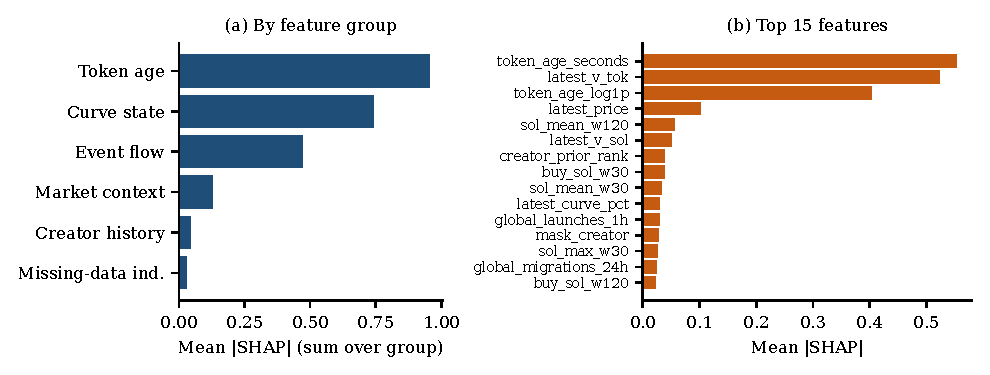
\includegraphics[width=\linewidth]{figures/fig_shap.pdf}
\caption{TreeSHAP attributions for the 300-second champion on 50,000 validation observations: (a) mean absolute attribution summed within each feature group; (b) the 15 most important individual features.}
\label{fig:shap}
\end{figure}

\subsection{Stability over time and the value of more data}

Across the days of the validation week, the champion's 300-second ROC-AUC ranged from 0.841 to 0.895 (Figure~\ref{fig:stability}a). When we trained the tuned configurations on the most recent 25\%, 50\%, 75\% and 100\% of the training period, validation PR-AUC at 60 seconds was highest with all the data for both LightGBM (0.077 at 25\% to 0.090 at 100\%) and XGBoost (0.080 to 0.091), and the curves had not leveled off (Figure~\ref{fig:stability}b). A longer history is the most promising way to improve these results.

\begin{figure}[t]
\centering
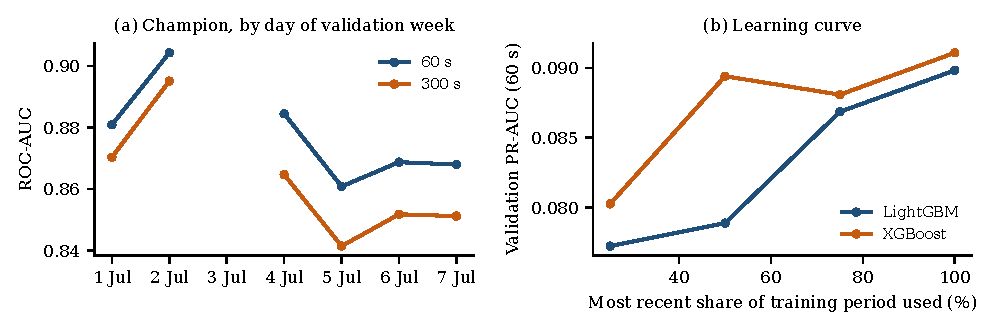
\includegraphics[width=\linewidth]{figures/fig_stability.pdf}
\caption{(a) Champion ROC-AUC on each day of the validation week; there are no data for 3 July. (b) Validation PR-AUC at 60 seconds when training on the most recent share of the training period.}
\label{fig:stability}
\end{figure}

\subsection{Predictable is not profitable}

A model that anticipates surges might seem to promise easy profits. Our data say otherwise (Table~\ref{tab:econ}). On the validation week, the median simple return over the five minutes after an observation was $-9.1\%$ across all eligible observations with a recorded return, and $-40.2\%$ (mean $-10.8\%$) for the champion's top 1\%. The same top-ranked observations had a median maximum favorable excursion of $+31.5\%$ and a median maximum adverse excursion of $-41.2\%$ over those five minutes: prices often rose first and then fell sharply. These are gross returns measured from the last trade price at $T$. They ignore fees and slippage and assume entry at exactly $T$; our data do not include prices for entries delayed by a realistic few seconds, and real outcomes would almost certainly be worse. The observations a model can most easily flag sit in the middle of bursts of activity that frequently reverse, which is what one would expect in a market where any obvious edge is competed away by faster participants.

\begin{table}[t]
\centering
\caption{Five-minute outcomes on the validation week (descriptive; gross of fees and slippage). MFE and MAE are the maximum favorable and adverse price excursions within five minutes.}
\label{tab:econ}
\tabsize
\begin{tabular}{lrcccc}
\toprule
 & & \multicolumn{2}{c}{5-min return} & Median & Median \\
\cmidrule(lr){3-4}
Observations & $n$ & Median & Mean & MFE & MAE \\
\midrule
All eligible observations & 516{,}383 & $-$9.1\% & $-$8.9\% & 1.1\% & $-$15.7\% \\
Champion top 1\% & 9{,}843 & $-$40.2\% & $-$10.8\% & 31.5\% & $-$41.2\% \\
\bottomrule
\end{tabular}

\end{table}
